%% Astronomy and Computing manuscript
%% Transient-glitch resilience for frozen DINGO-BNS
%% Single-file Overleaf upload: compile with pdfLaTeX (+ BibTeX if \usebibtextrue)
\documentclass[preprint,12pt]{elsarticle}

%% Toggle: false = embedded thebibliography (default, one-file Overleaf);
%%         true  = use refs.bib with elsarticle-num (upload both files).
\newif\ifusebibtex
\usebibtexfalse

\usepackage{amssymb,amsmath,amsfonts}
\usepackage{graphicx}
\usepackage{booktabs}
\usepackage{siunitx}
\usepackage{hyperref}
\usepackage{xcolor}
\usepackage{xspace}
\usepackage{enumitem}
\usepackage{natbib}

\journal{Astronomy and Computing}

\newcommand{\DINGOBNS}{DINGO-BNS\xspace}
\newcommand{\adapt}{\textsc{Adapt}\xspace}
\newcommand{\SNR}{\mathrm{SNR}}
\newcommand{\dL}{d_L}
\newcommand{\Mc}{\mathcal{M}}

\begin{document}

\begin{frontmatter}

\title{Transient-glitch resilience in neural gravitational-wave parameter estimation without network retraining}

\author{Jayant Kumar\corref{cor1}}
\ead{j.kumar16224@kgs.edu.pk}
\cortext[cor1]{Corresponding author.}
\affiliation{organization={Karachi Grammar School},
            addressline={Plot ST-19, Khayaban-e-Saadi, Clifton Block 5},
            city={Karachi},
            postcode={75600},
            state={Sindh},
            country={Pakistan}}

\begin{abstract}
Neural posterior estimators such as \DINGOBNS return complete binary neutron star (BNS) posteriors in about one second, but they are trained on stationary Gaussian noise and have no mechanism for signalling that an input lies outside that distribution.
We characterize how the official, frozen \DINGOBNS checkpoint responds to transient glitches overlapping the analysis segment, and we show that the failure can be mitigated by a preprocessing front-end that leaves the network weights untouched.
Placing synthetic and real glitches on a common loudness scale, the whitened optimal signal-to-noise ratio $\rho_w$, we find that the network is robust to ordinary glitches: 61 real O3 glitches from Gravity Spy injected at native loudness produce no failure below Omicron SNR $100$ ($\rho_w\lesssim150$), and a sweep of synthetic glitches shows the luminosity-distance posterior collapsing to a boundary of the network's prior in $50\%$ of cases only above $\rho_w\approx2.7\times10^{3}$.
That regime is real: $60\%$ of native Koi-Fish injections above Omicron SNR $300$ collapse the network, and $11\%$ of confidently classified O3 H1 Gravity Spy triggers exceed that loudness.
A detect--gate--rebuild front-end (STFT time-bin detection, Tukey gating, a matched-delta frequency-domain update, and retention of the original analysis ASDs) restores clean-like posteriors in $99\%$ of the 183 real-glitch cells, including every collapsed one, in $86\%$ of a 240-cell loud-glitch stress grid on GW170817, and in $92\%$ of a 160-cell synthetic BNS panel, with agreement on all 15 sampled parameters in a controlled case study.
Ablations show that the matched-delta update with the original ASDs is essential: replacing the packaged strain with the FFT of the gated strain recovers nothing.
A fixed-width oracle that knows the glitch time recovers fewer cells than the detector, establishing that residual failures are limited by gate extent rather than localization.
Software, the detector checkpoint, and archived results are released.
\end{abstract}

\begin{highlights}
\item Frozen \DINGOBNS is robust to ordinary glitches; distance collapses only above a measured loudness.
\item 11\% of confident O3 H1 Gravity Spy triggers are loud enough to collapse the network.
\item A detect--gate--rebuild front-end restores posteriors without retraining: 99\% on real glitches.
\item Matched-delta reconstruction with the original ASD is essential; FFT replacement recovers nothing.
\item Software, detector checkpoint, and archived results are released for reproduction.
\end{highlights}

\begin{keyword}
gravitational waves \sep binary neutron stars \sep neural posterior estimation \sep DINGO \sep signal gating \sep detector glitches
\end{keyword}

\end{frontmatter}

%% =====================================================================
\section{Introduction}
\label{sec:introduction}
%% =====================================================================

When two neutron stars merge, the window for finding their electromagnetic counterpart opens immediately and closes within hours.
The kilonova of GW170817 was found because a gravitational-wave sky map and distance estimate reached observers fast enough to tile the right region of the sky~\cite{Abbott2017gw170817,Abbott2017mma,Singer2016bayestar}.
As detector networks approach design sensitivity and binary neutron star (BNS) detections become routine, that latency budget is set by the time needed to turn strain data into a posterior, and conventional stochastic samplers require hours to days for a full BNS analysis~\cite{Morisaki2023rapid,Chaudhary2024latency}.

Amortized neural posterior estimation (NPE) removes this bottleneck by training a conditional density estimator to map strain data to posterior samples in a single forward pass~\cite{Cranmer2020sbi,Papamakarios2016mdn,Greenberg2019snpe,Papamakarios2021review,Durkan2019nsf}.
In gravitational-wave astronomy the programme has progressed from GW150914~\cite{Green2021npe} through DINGO for binary black holes~\cite{Dax2021dingo,Dax2022gnpe,Dax2023is,Wildberger2023psd} to \DINGOBNS, which returns a complete 17-parameter BNS posterior in about one second~\cite{Dax2025bns}.
The price of that speed is that the network only knows the data it was trained on: simulated signals in stationary Gaussian noise whose spectrum matches the measured power spectral density (PSD).

Real interferometer data are not like that.
Transient, non-Gaussian artefacts (glitches) occur often enough that of order one in five compact-binary candidates in the third observing run required some form of glitch mitigation~\cite{Nuttall2018transient,Davis2021detchar,Davis2022subtract,Glanzer2023gravityspy}.
For likelihood-based analyses the effect of a glitch is a bias that can be diagnosed, modelled, and subtracted~\cite{Powell2018glitchpe,Pankow2018mitigation,Payne2022gw200129,Ghonge2024efficacy,Macas2022localization}.
For an amortized network the situation is worse in a specific way: there is no likelihood to evaluate, so nothing in the sampler signals that the input is outside its training distribution, and the network cannot be retrained at event time against every glitch morphology.
We show below that the practical symptom, for the official \DINGOBNS checkpoint, is a luminosity-distance posterior that saturates at an edge of the network's prior, a wrong answer reported with high confidence, and we measure the glitch loudness at which it sets in.
Training-time remedies, such as augmenting the training set with glitches or redesigning the density estimator~\cite{Sun2024ttsf,Xiong2025robust}, are valuable but do not protect a checkpoint that is already deployed and whose weights must remain frozen for provenance and operational reasons.

This paper asks two operationally motivated questions.
First, how loud does a glitch have to be before a frozen \DINGOBNS posterior fails, and how often does real detector data cross that line?
Second, can a preprocessing front-end alone, with no change to the network, bring a contaminated input back inside the region where the posterior is trustworthy?
We answer the first with a measured threshold and a catalogue-level rate, and the second in the affirmative, finding that \emph{how} the excised data are written back into the network's input format matters more than the excision itself.
Our contributions are:
\begin{enumerate}[leftmargin=*,itemsep=0.25em]
\item We place synthetic and real glitches on a common loudness scale (whitened optimal SNR, $\rho_w$) and measure where the frozen network fails: no collapse below $\rho_w\approx100$, a $50\%$ collapse rate at $\rho_w\approx2.7\times10^{3}$, and collapse independent of where the glitch sits within the segment.
\item We test 61 real O3 Gravity Spy glitches at native loudness on GW170817: none below Omicron SNR 100 collapses the posterior, $60\%$ of loud Koi-Fish glitches (SNR $\geq300$) do, and $11\%$ of confidently classified O3 H1 triggers are that loud.
\item We introduce a detect--gate--rebuild front-end (STFT time-bin detection, Tukey gating, matched-delta frequency-domain reconstruction, retention of the original ASDs) that leaves the \DINGOBNS weights untouched and restores clean-like posteriors in $99\%$ of real-glitch cells, $86\%$ of a 240-cell loud-glitch stress grid, and $92\%$ of a synthetic BNS panel, including $96\%$ of cells whose morphology the detector never saw in training.
\item Through ablations we show that matched-delta reconstruction with the original ASD is the load-bearing ingredient, and we explain why the difference between it and a naive FFT rewrite is decisive.
\item Comparing detector-driven gates with a fixed-width oracle that knows the glitch time, we show that residual failures are governed by gate extent rather than localization; a clean-gate control quantifies the cost of a false trigger.
\item We release open software, the detector checkpoint, and archived results that reproduce every reported number.
\end{enumerate}
Section~\ref{sec:background} reviews neural BNS inference and glitch mitigation.
Section~\ref{sec:methods} specifies the front-end.
Section~\ref{sec:setup} describes the experimental design.
Section~\ref{sec:results} reports quantitative results.
Section~\ref{sec:discussion} discusses mechanism, limitations, and deployment, and Section~\ref{sec:conclusion} concludes.

%% =====================================================================

%% =====================================================================
\section{Background and related work}
\label{sec:background}
%% =====================================================================

\subsection{Bayesian inference and noise modelling}
\label{sec:bg-bayes}

Standard gravitational-wave parameter estimation treats the calibrated strain as a stationary Gaussian process with a frequency-dependent PSD and evaluates a Whittle likelihood against a waveform model~\cite{Abbott2020guide}.
PSD estimation choices affect inferred parameters~\cite{Chatziioannou2019psd,Talbot2020psd}, and violations of stationarity or Gaussianity, including short bursts and slow drifts, invalidate credible intervals even when point estimates remain approximately unbiased~\cite{Edy2021mismodel,Mozzon2020dynamic,Zackay2021nongaussian}.
Public guides, catalogues, and open data releases document these assumptions and the tools used to enforce them in practice~\cite{Abbott2020guide,Abbott2019gwtc1,Abbott2021opendata,Abbott2023opendata,Macleod2021gwpy,Ashton2019bilby}.

\subsection{Neural posterior estimation and \DINGOBNS}
\label{sec:bg-npe}

NPE trains a conditional normalizing flow $q_\phi(\theta\mid d)$ to approximate the Bayesian posterior $p(\theta\mid d)$ using simulated pairs $(\theta,d)$ drawn from the prior and the forward model~\cite{Cranmer2020sbi,Papamakarios2021review}.
DINGO embeds whitened frequency-domain strain and conditions on the PSD, enabling amortized inference at second-scale latency~\cite{Dax2021dingo,Dax2022gnpe}.
\DINGOBNS extends this programme to long BNS signals with complete 17-parameter inference~\cite{Dax2025bns}.
Importance sampling can diagnose and correct network residuals when a tractable likelihood is available~\cite{Dax2023is}, and latent PSD models can extend temporal coverage~\cite{Wildberger2023psd}.
None of these mechanisms, however, is a substitute for bringing an out-of-distribution glitch back into the training support of a frozen checkpoint.

\subsection{Transient noise in ground-based detectors}
\label{sec:bg-glitches}

Glitches arise from instrumental and environmental couplings and exhibit diverse time--frequency morphologies~\cite{Abbott2016noise,Nuttall2018transient,Davis2021detchar}.
Citizen-science and machine-learning catalogues such as Gravity Spy provide morphological taxonomies used throughout detector characterization~\cite{Zevin2017gravityspy,Bahaadini2018,Glanzer2023gravityspy}.
Blip-like short bursts and scattered-light arches are particularly relevant to compact-binary analyses~\cite{Cabero2019blip,Soni2021scattered}.
During O3, of order 20\% of candidates required some form of glitch mitigation~\cite{Davis2022subtract}, and nearby glitches can bias low-latency sky maps~\cite{Macas2022localization}.

\subsection{Mitigation for likelihood-based parameter estimation}
\label{sec:bg-mitigation}

Likelihood-based pipelines mitigate glitches by gating~\cite{Zackay2021nongaussian,Usman2016pycbc}, by joint wavelet modelling of signal and glitch (BayesWave)~\cite{Cornish2015bayeswave,Pankow2018mitigation,Hourihane2022overlap,Davis2022subtract,Ghonge2024efficacy}, by parametric or data-driven glitch bases~\cite{Merritt2021glitschen,Malz2025joint}, or by modifying the noise model itself~\cite{Ashton2023gp}.
These methods are powerful but typically assume an evaluable likelihood and often incur minutes-to-hours of additional compute; acceptable offline, less so when the downstream estimator is an amortized network whose value proposition is second-scale sampling.

\subsection{Glitches and neural parameter estimation}
\label{sec:bg-neural-glitch}

Two recent lines of work train normalizing flows to remain accurate under glitch contamination, either by time--spectral fusion architectures~\cite{Sun2024ttsf} or by studying robustness to sine-Gaussian contaminants without explicit deglitching~\cite{Xiong2025robust}.
Malz and Veitch~\cite{Malz2025joint} instead learn a Gravity Spy-informed glitch prior and sample signal and glitch jointly inside Bilby.
Convolutional classifiers for glitch morphology~\cite{Razzano2018cnn,George2018dnn} address detection and categorization rather than posterior recovery.
Our setting is complementary and deliberately constrained: the \DINGOBNS production weights are frozen; only a lightweight detector is trained; and mitigation is a data-domain front-end that restores inputs compatible with the existing network.

%% =====================================================================
\section{Methods}
\label{sec:methods}
%% =====================================================================

\subsection{Problem statement}
\label{sec:problem}

Let $d$ denote the frequency-domain event package consumed by \DINGOBNS (whitened strain and ASDs for each interferometer) and let $q_\phi(\theta\mid d)$ be the frozen neural posterior.
A short glitch $g$ overlapping the analysis segment produces a contaminated package $d_g$ for which $q_\phi(\theta\mid d_g)$ can differ qualitatively from $q_\phi(\theta\mid d)$.
In our diagnostics the dominant symptom is \emph{saturation}: the luminosity-distance marginal, whose clean 90\% interval spans roughly $19$--$45\,\mathrm{Mpc}$ for GW170817, collapses to a narrow spike at one boundary of the network's training prior, $[10,100]\,\mathrm{Mpc}$ (Section~\ref{sec:results-gw170817}).
The network is not returning a biased distance; it is returning the edge of what it is allowed to say, with a credible interval that is far too narrow.
We seek a map $d_g\mapsto \tilde d$ such that $q_\phi(\theta\mid \tilde d)\approx q_\phi(\theta\mid d)$ without modifying $\phi$.

\subsection{A common loudness scale}
\label{sec:loudness}

To compare synthetic injections, real glitches, and catalogue statistics we express every injected glitch $g$ by its whitened optimal signal-to-noise ratio in the injected interferometer,
\begin{equation}
\label{eq:rhow}
\rho_w^2 = 4\int_{f_{\min}}^{f_{\max}} \frac{|\tilde g(f)|^2}{S_n(f)}\,\mathrm{d}f ,
\end{equation}
evaluated on the packaged frequency grid with the GW170817 analysis PSD $S_n$.
This is the matched-filter SNR the glitch would have if it were the template, and it is the quantity the whitened network input actually sees.
Gravity Spy reports an Omicron SNR for each trigger~\cite{Zevin2017gravityspy,Glanzer2023gravityspy}; on the real glitches we injected, $\rho_w$ is larger than the Omicron SNR by a median factor of $2.1$ (from $1.8$ for blips to $3.7$ for whistles), so the two axes can be read against each other to within a factor of a few.

\subsection{Pipeline overview}
\label{sec:pipeline}

Figure~\ref{fig:pipeline} summarizes the front-end.
Contaminated time-domain strain is transformed to a whitened STFT, scored by a convolutional time-bin detector, converted to Tukey gate windows, excised in the time domain, and rewritten into the frequency-domain package by a matched-delta update that preserves the original analysis ASDs.
The rebuilt package is passed to the unchanged \DINGOBNS sampler.

\begin{figure}[t]
\centering
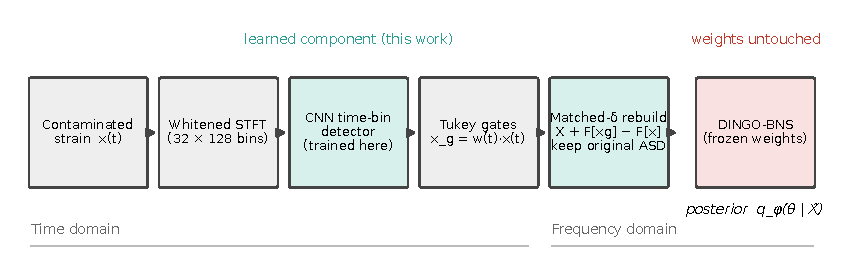
\includegraphics[width=\linewidth]{figures/fig1_pipeline.pdf}
\caption{The glitch-resilience front-end.
Contaminated strain is scored by a small convolutional detector on its whitened spectrogram, gated in the time domain, and written back into the frequency-domain event package by a matched-delta update that keeps the original analysis ASD.
Only the detector is trained; the official \DINGOBNS weights remain frozen.}
\label{fig:pipeline}
\end{figure}

\subsection{STFT glitch detector}
\label{sec:detector}

For each interferometer we form a whitened spectrogram on a fixed grid of $T=32$ time bins and $F=128$ frequency bins (analysis crop $\approx 4\,\mathrm{s}$, $n_{\mathrm{fft}}=2048$, hop $256$ samples at $4096\,\mathrm{Hz}$).
A compact convolutional network maps the multi-detector spectrogram stack to per-interferometer, per-time-bin logits.
Architecture details and training hyperparameters are given in \ref{app:detector}.
Operating thresholds are calibrated to a target clean false-positive rate of $1\%$ on held-out clean crops; at event time an optional stricter threshold (used in the GW170817 stress grid) further suppresses clean triggers.
Positive time bins are dilated to Tukey windows of half-width $0.4\,\mathrm{s}$ (default).

\subsection{Tukey gating}
\label{sec:gating}

Given gate windows $\{(t_{s,i},t_{e,i})\}$, we form multiplicative weights $w(t)\in[0,1]$ that equal unity outside gates and follow a Tukey taper (shape parameter $\alpha=0.5$) inside each window~\cite{Harris1978windows}.
Gated time-domain strain is $x_{\mathrm{g}}(t)=w(t)\,x(t)$.
Detector-driven gates are built by dilating \emph{every} positive STFT time bin by $\pm0.4\,\mathrm{s}$ and merging overlapping windows, so their total extent grows with the duration of the detected excess.

As a diagnostic we also construct a \emph{centred fixed-width oracle}: a single gate of the same $\pm0.4\,\mathrm{s}$ half-width centred exactly on the true injection time.
The oracle has perfect localization but a fixed extent, so comparing it with the detector-driven gate separates two possible causes of failure, mislocalization and insufficient excision.
It is never used as the primary method.

\subsection{Matched-delta frequency-domain reconstruction}
\label{sec:matched-delta}

Let $X(f)$ be the packaged frequency-domain strain for a gated interferometer and let $\mathcal{F}$ denote the analysis Tukey-windowed real FFT consistent with the \DINGOBNS event packaging.
The matched-delta update replaces $X$ by
\begin{equation}
\label{eq:matched-delta}
\tilde X(f) = X(f) + \mathcal{F}[x_{\mathrm{g}}](f) - \mathcal{F}[x](f),
\end{equation}
i.e.\ it adds the Fourier transform of the gated-minus-ungated residual rather than overwriting $X$ with $\mathcal{F}[x_{\mathrm{g}}]$.
The distinction deserves emphasis because the two operations are algebraically equivalent \emph{if} $\mathcal{F}$ reproduces the packaging transform exactly: were $X=\mathcal{F}[x]$, Eq.~\eqref{eq:matched-delta} would reduce to $\tilde X=\mathcal{F}[x_{\mathrm{g}}]$.
In practice $\mathcal{F}$ is only an approximation to the sequence of windowing, resampling, band-limiting, and calibration steps that produced the packaged $X$, so $X-\mathcal{F}[x]=\varepsilon(f)$ is small but non-zero.
Full replacement discards $\varepsilon$; the matched-delta update carries it through unchanged and applies only the \emph{difference} $\mathcal{F}[x_{\mathrm{g}}]-\mathcal{F}[x]$, which is dominated by the excised glitch and is insensitive to a common mismatch in $\mathcal{F}$ to first order.
In the injection studies, where $X=\mathcal{F}_{\mathrm{pkg}}[x_{\mathrm{clean}}]+\mathcal{F}_{\mathrm{pkg}}[g]$, the update removes the gated portion of $g$ while leaving every packaging convention the network was trained on intact.
The ablation arm \texttt{fft\_replace}, which sets $\tilde X=\mathcal{F}[x_{\mathrm{g}}]$, discards $\varepsilon$ and fails in every tested cell (Section~\ref{sec:results-ablation}); the size of that effect is itself evidence that $\varepsilon$, although invisible in a whitened strain plot, lies well outside the tolerance of the frozen network.

\subsection{ASD policy}
\label{sec:asd}

After reconstruction we restore the original analysis ASDs that accompany the event package.
Welch estimates recomputed on the gated segment~\cite{Welch1967} are \emph{not} retained: they encode the gate as a spectral feature and drive residual collapse in ablation.
This choice is the frequency-domain analogue of insisting that whitening statistics match those seen in training~\cite{Chatziioannou2019psd,Talbot2020psd,Wildberger2023psd}.

\subsection{Frozen sampler}
\label{sec:sampler}

Posterior samples are drawn with the official GW170817 \DINGOBNS demonstration checkpoint via the unchanged \texttt{GWSamplerGNPE} interface.
No embedding weights, flow parameters, or PE heads are fine-tuned.
The only learned component contributed here is the STFT detector checkpoint distributed with the accompanying software.

%% =====================================================================
\section{Experimental setup}
\label{sec:setup}
%% =====================================================================

\subsection{Data and assets}
\label{sec:data}

All GW170817 experiments use the public open-data packaging and the official \DINGOBNS demonstration model~\cite{Abbott2017gw170817,Abbott2021opendata,Abbott2023opendata,Dax2025bns}.
Synthetic BNS events are generated with the same domain conventions (segment duration, sampling rate, frequency grid, and ASD handling) so that the frozen checkpoint remains applicable.
Strain handling uses GWpy and the scientific Python stack~\cite{Macleod2021gwpy,Harris2020numpy,Virtanen2020scipy,Paszke2019pytorch}.

\subsection{Glitch families and severity}
\label{sec:glitches}

We inject morphologically diverse synthetic glitches into a single interferometer (H1 unless noted):
held-in families \{\texttt{sine\_gaussian}, \texttt{broadband\_burst}, \texttt{whistle}, \texttt{scattered\_light}, \texttt{glitch\_train}\} used in detector training, and held-out families \{\texttt{ringing}, \texttt{double\_blip}, \texttt{narrowband\_tone}\}.
Amplitude is set by an in-band amplitude ratio relative to the local raw-strain noise, with severity midpoints $\{3,6,10\}$; \ref{app:glitch} lists parameter ranges.
Because raw in-band RMS is dominated by the low-frequency noise wall, this convention produces very loud glitches on the whitened scale: median $\rho_w$ is $4.2\times10^{3}$, $7.3\times10^{3}$, and $1.0\times10^{4}$ at the three severities (range $1.5\times10^{2}$--$6.4\times10^{4}$), and the official-control sine-Gaussian has $\rho_w=4.3\times10^{3}$.
The synthetic panels are therefore a stress test of the \emph{loud} tail of the glitch population (Section~\ref{sec:results-threshold}), not of typical glitches.
ASD policies alternate between retaining the stationary analysis ASD and recomputing a Welch ASD on the contaminated segment, so that collapse and recovery can be attributed to strain versus noise-spectrum mismodelling.

\paragraph{Loudness sweep}
To locate the failure threshold we inject sine-Gaussians and broadband bursts into the GW170817 H1 segment at target $\rho_w$ values log-spaced from $10$ to $10^{4}$ (eight levels, five seeds, plus twenty additional cells at each of $\rho_w\in\{10,30,100\}$), with the injection time drawn uniformly in $[-1.5,-0.3]\,\mathrm{s}$ relative to the trigger.

\paragraph{Real Gravity Spy glitches}
We select H1 triggers from the O3 Gravity Spy classifications~\cite{Glanzer2023gravityspy} with machine-learning confidence $\geq0.95$ and duration $\leq3\,\mathrm{s}$, in four Omicron-SNR bins ($[8,30)$, $[30,100)$, $[100,300)$, $[300,\infty)$) for five morphologies (Blip, Koi Fish, Scattered Light, Tomte, Whistle), taking the highest-confidence triggers in each bin; 72 were selected, 70 fetched from GWOSC (two fell in data gaps), and 61 yielded a usable excerpt.
For each, $8\,\mathrm{s}$ of open strain centred on the trigger is whitened with a PSD from its own off-trigger portion, cut to the trigger duration (at least $\pm0.5\,\mathrm{s}$) with a Tukey taper, reduced to a glitch-only estimate by thresholding its STFT at eight times the per-frequency off-trigger median power, re-coloured with the GW170817 H1 analysis ASD, and added to the H1 analysis segment at three injection times per glitch ($183$ cells).
Injection is at \emph{native} loudness, i.e.\ the same whitened energy the glitch had in O3; no rescaling is applied.
Five trigger-free O3 excerpts processed identically (without thresholding) serve as a noise-only control.
Working in the whitened domain is necessary because a Gravity Spy blip at Omicron SNR 20 is not measurable as a raw in-band RMS excess at all.

\subsection{Evaluation panels}
\label{sec:panels}

\begin{description}[style=nextline,leftmargin=1.2em]
\item[GW170817 stress grid.]
Eight families $\times$ three severities $\times$ two ASD policies $\times$ five seeds yield $N=240$ cells.
A clean reference posterior ($n=512$ samples) anchors recovery criteria.
\item[Synthetic BNS panel.]
Locked injections that pass a known-answer test (KAT) against the frozen sampler; $N=160$ glitch cells across four families and two severities.
\item[Loudness sweep.]
$N=139$ cells on GW170817 across $\rho_w=10$--$10^{4}$ (Section~\ref{sec:glitches}); arms: poisoned and gated.
\item[Real Gravity Spy panel.]
$N=183$ native-loudness cells from 61 O3 H1 glitches plus 5 noise-only cells; arms: poisoned, gated, and centred oracle.
\item[Clean-gate cost control.]
$N=25$ forced $\pm0.4\,\mathrm{s}$ gates on glitch-free GW170817 data (20 on H1 at injection times uniform in $[-2.0,-0.2]\,\mathrm{s}$; 5 on H1 and L1 simultaneously), passed through the full front-end and compared with the clean posterior.
\item[Method hardening / ablation.]
$N=16$ cells comparing five arms: \texttt{poison\_welch}, \texttt{glitch\_orig\_asd}, \texttt{gate\_welch}, \texttt{adapt\_full}, and \texttt{fft\_replace}.
\item[Clean false-positive audit.]
Fifty clean GW170817 draws at the event-level threshold; the detector must not fire.
A separate no-glitch pass through the full front-end confirms that, when no gate fires, the rebuilt package is bit-identical to the input.
\end{description}

\subsection{Success criteria}
\label{sec:criteria}

A poisoned posterior is labelled \emph{collapsed} if the 90\% credible interval on $\dL$ has upper edge below $15\,\mathrm{Mpc}$ or lower edge above $90\,\mathrm{Mpc}$ (relative to the GW170817 clean median $\approx 34\,\mathrm{Mpc}$).
The two thresholds correspond to the collapse spikes observed at the prior boundaries.
A gated posterior \emph{recovers} if its $\dL$ median lies in $[20,50]\,\mathrm{Mpc}$ and within $10\,\mathrm{Mpc}$ of the clean median, and its 90\% credible interval overlaps the clean interval.
These are deliberately coarse, $\dL$-only criteria chosen to separate collapse from non-collapse across hundreds of cells with $n=512$ samples each; on successful cells the actual median offsets are far smaller (mean $1$--$1.4\,\mathrm{Mpc}$, reported per panel).
For the official-control case study we additionally compute Jensen--Shannon (JS) divergences~\cite{Lin1991jsd} between clean and gated one-dimensional marginals for all 15 sampled parameters and require $\mathrm{JS}<0.02\,\mathrm{nat}$ on the core set $\{\Mc,q,\dL,\theta_{JN},t_{\mathrm{c}}\}$.
All criteria are implemented in the released drivers; the reported rates are read directly from the archived CSVs.

\subsection{Software and reproducibility}
\label{sec:repro}

Example drivers, configuration hashes, and archived JSON/CSV summaries are released with the accompanying repository (\ref{app:repro}).
Reported metrics are taken from the full (non-smoke) archived runs under \texttt{results/}.

%% =====================================================================
\section{Results}
\label{sec:results}
%% =====================================================================

\subsection{Where the frozen network fails}
\label{sec:results-threshold}

Figure~\ref{fig:threshold} shows the poisoned collapse rate and the gated recovery rate as a function of injected loudness on the GW170817 segment.
Below $\rho_w\approx100$ no cell collapses (69 cells at $\rho_w\in\{10,30,100\}$).
Collapse appears at $\rho_w\approx200$ ($10\%$), reaches $30\%$ at $\rho_w\approx500$--$1400$, $60\%$ at $\rho_w\approx3700$, and $80\%$ at $10^{4}$; the interpolated $50\%$ crossing is $\rho_w\approx2.7\times10^{3}$ ($2.3\times10^{3}$ for broadband bursts, $6.1\times10^{3}$ for sine-Gaussians).
Collapse does not depend on where the glitch sits: at $\rho_w>3000$, pooling the sweep with the stress grid of Section~\ref{sec:results-gw170817} (194 cells), the collapse rate is $56\%$ for injections within $1\,\mathrm{s}$ of the trigger and $53\%$ further away ($p=0.75$).
The failure is therefore governed by how much whitened power the glitch adds, not by whether it overlaps the loudest part of the inspiral.
Across the whole sweep the gated front-end recovers $97\%$ of cells and $90\%$ of collapsed cells.
At the low end, where the detector fires on $0\%$ of cells at $\rho_w=10$ and about $65\%$ at $\rho_w=30$, gated recovery is $100\%$ and the mean $\dL$-median offset is $0.5$--$1.6\,\mathrm{Mpc}$: a gate applied to a glitch that was never going to hurt costs little.

\begin{figure}[t]
\centering
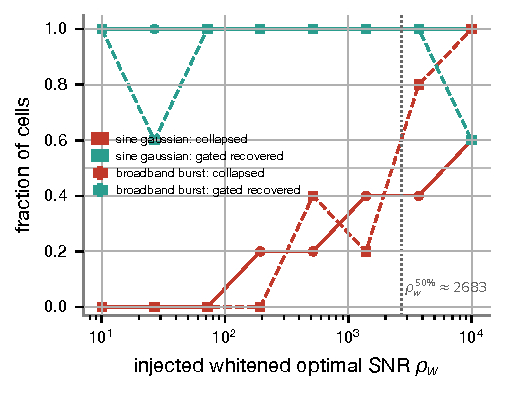
\includegraphics[width=0.62\linewidth]{figures/fig9_threshold.pdf}
\caption{Loudness sweep on GW170817.
Poisoned collapse rate and gated recovery rate as a function of the whitened optimal SNR $\rho_w$ of the injected glitch, for sine-Gaussians and broadband bursts (grid points within a factor of 1.5 pooled; 139 cells).
The shaded band is the $\rho_w$ range of real O3 Gravity Spy glitches with Omicron SNR 9--30.
The dotted line marks the interpolated $50\%$ collapse point.}
\label{fig:threshold}
\end{figure}

\subsection{Real O3 glitches at native loudness}
\label{sec:results-real}

Figure~\ref{fig:real} and Table~\ref{tab:real} report the 183 real-glitch cells.
The picture is consistent with the sweep.
Across the two lower Omicron-SNR bins (123 cells, 41 glitches; $\rho_w\approx40$--$70$) no cell collapses.
In the $[100,300)$ bin ($\rho_w\approx190$) $18\%$ collapse, and in the $[300,\infty)$ bin ($\rho_w\approx560$) $60\%$ collapse.
Morphology matters: every collapse is a Koi-Fish glitch ($53\%$ of Koi-Fish cells at SNR $100$--$300$ and $60\%$ above $300$), whereas blips, whistles, tomtes, and scattered light never collapse the network at the loudness they reach in this sample.
The five noise-only controls do not collapse, so the effect is not an artefact of transplanted O3 noise.

The front-end recovers $99\%$ of cells ($181/183$), including every one of the 17 collapsed cells; the mean $\dL$-median offset on successes is $1.0\,\mathrm{Mpc}$.
The two failures are both scattered-light cells whose poisoned posterior was already fine and where the gate over-excised, pulling the $\dL$ median to $18$ and $22\,\mathrm{Mpc}$; the centred oracle, with its narrower support, recovers both.
The detector fires on $87\%$ of cells overall, rising from $85\%$ in the quietest bin to $100\%$ above SNR 300; the cells it does not fire on are quiet ones that pass through unchanged and, being non-collapsed, count as recovered.
The centred oracle recovers $90\%$, losing to the detector on every morphology, for the reason given in Section~\ref{sec:results-oracle}.

\begin{figure}[t]
\centering
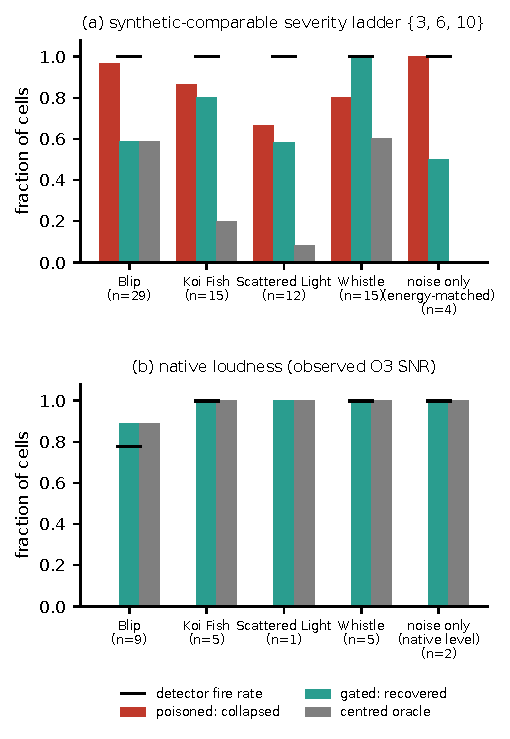
\includegraphics[width=\linewidth]{figures/fig8_real_glitches.pdf}
\caption{Real O3 H1 Gravity Spy glitches injected into GW170817 at native loudness (183 cells).
Left: by Omicron-SNR bin, with the median injected $\rho_w$ of each bin.
Right: by morphology, with the five noise-only control cells.
Bars are poisoned collapse, detector-gated recovery, and centred-oracle recovery; ticks are the detector fire rate.}
\label{fig:real}
\end{figure}

\begin{table}[t]
\centering
\caption{Real Gravity Spy panel by Omicron-SNR bin ($N=183$ native-loudness cells).
$\rho_w$ is the median whitened optimal SNR of the injected excerpts in the bin.}
\label{tab:real}
\footnotesize
\setlength{\tabcolsep}{4.5pt}
\begin{tabular}{lccccccc}
\toprule
SNR bin & Glitches & $N$ & $\rho_w$ & Collapse & Gated rec. & Oracle rec. & Det. fire \\
\midrule
$[8,30)$      & 18 & 54 & 42  & 0.000 & 1.000 & 0.926 & 0.852 \\
$[30,100)$    & 23 & 69 & 71  & 0.000 & 0.971 & 0.899 & 0.841 \\
$[100,300)$   & 15 & 45 & 186 & 0.178 & 1.000 & 0.933 & 0.911 \\
$[300,\infty)$&  5 & 15 & 560 & 0.600 & 1.000 & 0.733 & 1.000 \\
\midrule
All           & 61 & 183 & 80 & 0.093 & 0.989 & 0.902 & 0.874 \\
Noise only    & 5  & 5   & 64 & 0.000 & 1.000 & 1.000 & 1.000 \\
\bottomrule
\end{tabular}
\end{table}

\paragraph{Prevalence in the O3 catalogue}
Among the $132{,}065$ O3 H1 Gravity Spy triggers with confidence $\geq0.95$, the median Omicron SNR is $13$, but the distribution has a long tail: $11.0\%$ exceed SNR $300$, $7.4\%$ exceed $10^{3}$, and $5.0\%$ exceed $2\times10^{3}$.
The tail is dominated by two classes, ``Extremely Loud'' ($14{,}894$ triggers, $89\%$ above SNR 300) and Koi Fish ($9{,}683$ triggers, $13\%$ above 300); blips, whistles, scattered light, and tomtes essentially never reach it.
The synthetic stress grid of the following sections, with $\rho_w\sim10^{3}$--$10^{4}$, is therefore a test of a regime that roughly one in ten confidently classified O3 glitches occupies, not a hypothetical one.

\subsection{Qualitative failure and recovery}
\label{sec:results-qual}

Figure~\ref{fig:example} illustrates a representative H1 sine-Gaussian injection into the GW170817 package.
The whitened spectrogram shows a compact excess; the detector marks a contiguous time support; Tukey gates zero that support; and the matched-delta rebuild restores a frequency-domain package on which \DINGOBNS again yields an extended $\dL$ marginal.
Figure~\ref{fig:posteriors} contrasts clean, poisoned, and gated one-dimensional posteriors in the official-control case study (an H1 sine-Gaussian at $f_0=100\,\mathrm{Hz}$, $Q=5$, $1\,\mathrm{s}$ before the trigger, $\rho_w=4.3\times10^{3}$).
The poisoned run collapses to $\dL\approx10\,\mathrm{Mpc}$ with a 90\% interval of width $0.65\,\mathrm{Mpc}$, against a clean interval spanning $19$--$45\,\mathrm{Mpc}$.
The gated run overlaps the clean reference on every one of the 15 sampled parameters (Table~\ref{tab:js}); the largest JS divergence, $0.012\,\mathrm{nat}$, occurs for the secondary spin magnitude $a_2$, and the $\dL$ median shifts by $-0.3\,\mathrm{Mpc}$.
The importance-sampling efficiency of the gated package ($8.5\%$) is comparable to that of the clean package ($11.1\%$), indicating that the rebuilt input remains close to the network's training support rather than merely producing a plausible-looking marginal.

\begin{table}[t]
\centering
\caption{Official-control case study: one-dimensional JS divergence (nat) between the clean and gated posteriors, and whether the 90\% credible intervals overlap, for all 15 sampled parameters.
Core parameters used in the recovery criterion are marked with $\ast$.}
\label{tab:js}
\small
\begin{tabular}{lcc@{\hskip 1.5em}lcc}
\toprule
Parameter & JS & Overlap & Parameter & JS & Overlap \\
\midrule
$\Mc$ $\ast$              & 0.0072 & \checkmark & $\phi_{12}$          & 0.0057 & \checkmark \\
$\delta\Mc$               & 0.0073 & \checkmark & $\phi_{JL}$          & 0.0070 & \checkmark \\
$q$ $\ast$                & 0.0080 & \checkmark & $\theta_{JN}$ $\ast$ & 0.0070 & \checkmark \\
$a_1$                     & 0.0098 & \checkmark & $\psi$               & 0.0074 & \checkmark \\
$a_2$                     & 0.0118 & \checkmark & $t_{\mathrm{c}}$ $\ast$ & 0.0049 & \checkmark \\
$\theta_1$                & 0.0085 & \checkmark & $\Lambda_1$          & 0.0014 & \checkmark \\
$\theta_2$                & 0.0098 & \checkmark & $\Lambda_2$          & 0.0014 & \checkmark \\
$\dL$ $\ast$              & 0.0066 & \checkmark &                      &        &            \\
\bottomrule
\end{tabular}
\end{table}

\begin{figure}[t]
\centering
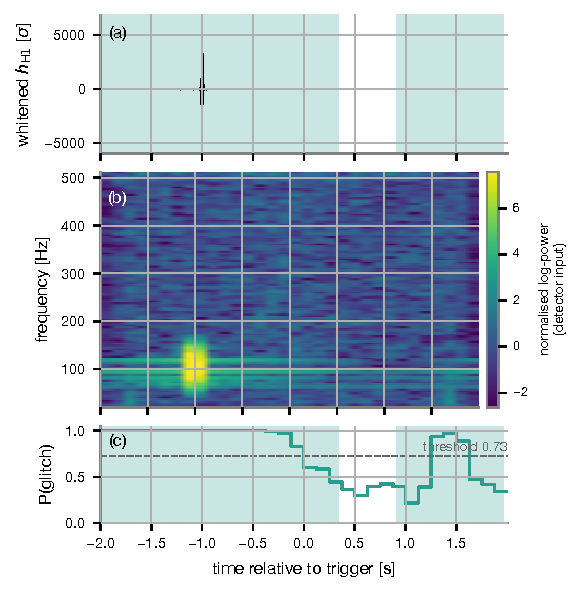
\includegraphics[width=0.6\linewidth]{figures/fig2_injection_gate.pdf}
\caption{Example glitch injection, detection, and gating on the GW170817 H1 analysis crop.
Top: whitened strain with the injected sine-Gaussian and the Tukey gate window (shaded).
Middle: the whitened spectrogram seen by the detector.
Bottom: per-time-bin detector probability with the event-level threshold.}
\label{fig:example}
\end{figure}

\begin{figure}[t]
\centering
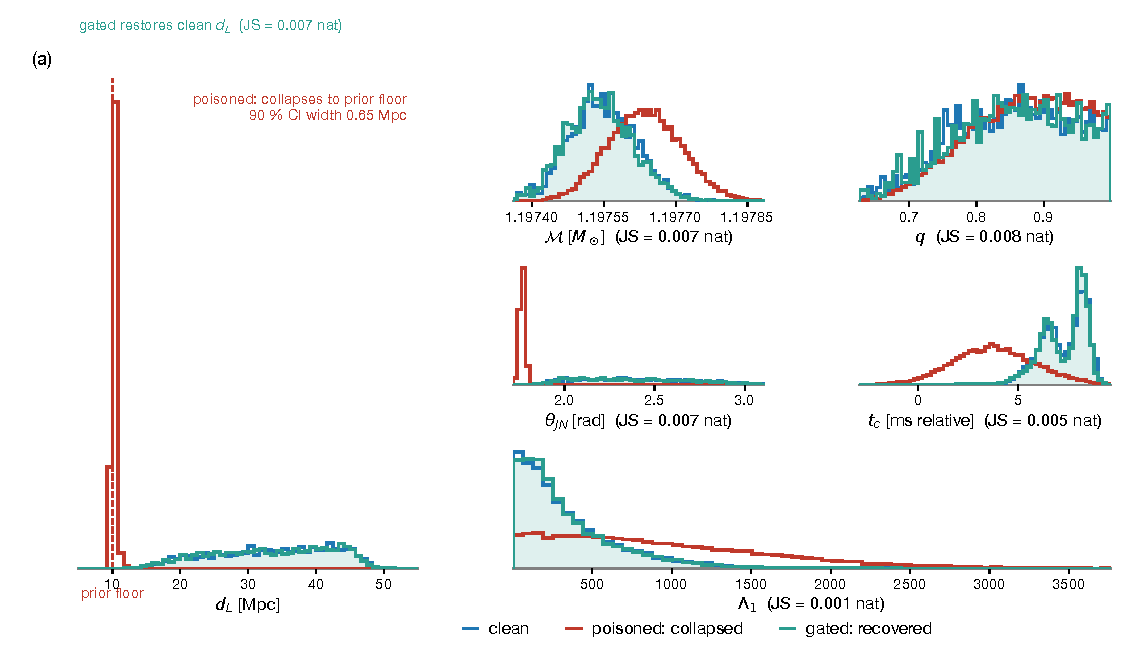
\includegraphics[width=\linewidth]{figures/fig3_posteriors.pdf}
\caption{Posterior comparison for the official-control case study.
One-dimensional marginals of $\dL$, $\Mc$, $q$, $\theta_{JN}$, $t_{\mathrm{c}}$, and $\Lambda_1$ for the clean (importance-sampled official result), poisoned, and gated runs.
Poisoning drives $\dL$ into a spike at the $10\,\mathrm{Mpc}$ prior floor; the gated reconstruction restores the clean support on every parameter.}
\label{fig:posteriors}
\end{figure}

\subsection{GW170817 loud-glitch stress grid}
\label{sec:results-gw170817}

The stress grid probes the loud regime ($\rho_w$ median $4$--$10\times10^{3}$) across eight morphologies.
Poisoned collapse occurs in $46.3\%$ of the 240 cells (Table~\ref{tab:gw170817}), consistent with the sweep at these loudnesses.
Of the 111 collapsed cells, 90 saturate at the $10\,\mathrm{Mpc}$ prior floor and 21 at the $100\,\mathrm{Mpc}$ ceiling; in no case does the poisoned posterior land at an intermediate distance with a broad interval, which is the signature one would expect from a mild bias.
Collapse is more frequent when the stationary analysis ASD is retained ($60.0\%$) than when a Welch ASD is recomputed on the contaminated segment ($32.5\%$), because the latter partially absorbs the glitch power into the whitening; but as the ablation shows, that route does not lead to recovery either.

The gated front-end recovers $85.8\%$ of all cells and $77.5\%$ of the cells that had collapsed.
Held-out families, whose morphologies the detector never saw during training, recover at $95.6\%$, compared with $80.0\%$ for held-in families; the pipeline is therefore not memorizing training morphologies, and the held-in figure is dominated by the single hardest family.
Recovery declines mildly with severity ($90.0\%$, $86.3\%$, $81.3\%$ at midpoints 3, 6, 10) and is comparable under stationary and Welch ASD policies ($84.2\%$ vs.\ $87.5\%$).
On successful cells the mean absolute offset of the $\dL$ median from the clean reference is $1.1\,\mathrm{Mpc}$, well inside the clean 90\% interval width of $26\,\mathrm{Mpc}$.
The weakest family is \texttt{scattered\_light} ($50\%$ gated recovery): long, low-frequency arches often exceed the gate extent, so residual power remains after gating.
Figure~\ref{fig:heatmap} summarizes collapse and recovery by family and severity.

\begin{table}[t]
\centering
\caption{GW170817 stress grid ($N=240$).
Gated recovery is the fraction of cells whose post-front-end posterior matches the clean reference under the criteria of Section~\ref{sec:criteria}.
Oracle recovery uses a single $\pm0.4\,\mathrm{s}$ gate centred on the true injection time (perfect localization, fixed extent).
Held-out families ($\dagger$) were not seen by the detector in training.}
\label{tab:gw170817}
\begin{tabular}{lcccc}
\toprule
Family & $N$ & Poison collapse & Gated recovery & Oracle recovery \\
\midrule
\texttt{broadband\_burst} & 30 & 0.833 & 0.767 & 0.967 \\
\texttt{double\_blip}$^\dagger$     & 30 & 0.367 & 0.900 & 0.967 \\
\texttt{glitch\_train}    & 30 & 0.467 & 0.967 & 0.933 \\
\texttt{narrowband\_tone}$^\dagger$ & 30 & 0.167 & 1.000 & 0.600 \\
\texttt{ringing}$^\dagger$          & 30 & 0.633 & 0.967 & 0.567 \\
\texttt{scattered\_light} & 30 & 0.467 & 0.500 & 0.233 \\
\texttt{sine\_gaussian}   & 30 & 0.233 & 0.967 & 0.900 \\
\texttt{whistle}          & 30 & 0.533 & 0.800 & 0.533 \\
\midrule
Overall                   & 240 & 0.463 & 0.858 & 0.713 \\
Held-in                   & --- & --- & 0.800 & --- \\
Held-out                  & --- & --- & 0.956 & --- \\
\bottomrule
\end{tabular}
\end{table}

\begin{figure}[t]
\centering
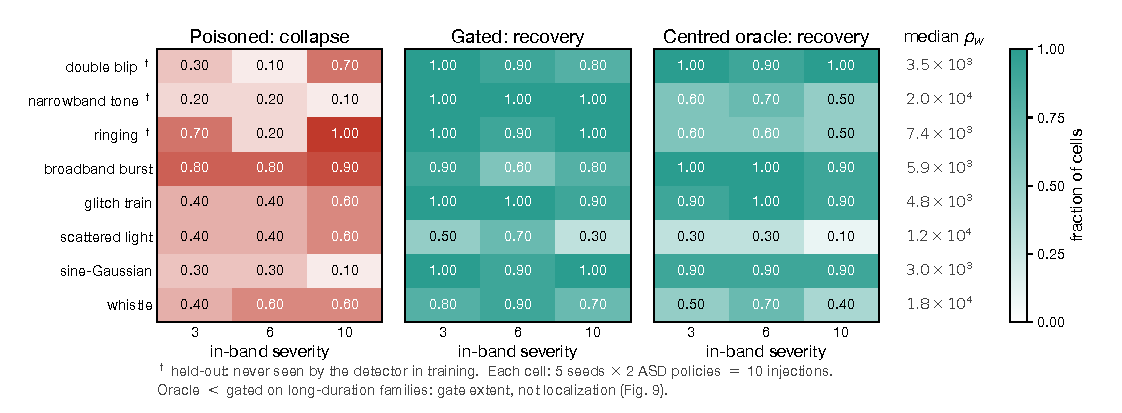
\includegraphics[width=\linewidth]{figures/fig4_gw170817_heatmap.pdf}
\caption{GW170817 stress grid by family and severity: poisoned collapse rate (left), detector-driven gated recovery (centre), and centred fixed-width oracle recovery (right).
Each cell aggregates five seeds and two ASD policies.
The detector-driven gate matches or exceeds the oracle on every family whose glitches outlast the oracle window (Section~\ref{sec:results-oracle}).}
\label{fig:heatmap}
\end{figure}

A clean false-positive audit of 50 draws at the event threshold yields zero fires, and a no-glitch pass through the full front-end reproduces the input package bit-exactly.

\subsection{Localization versus extent: the oracle comparison}
\label{sec:results-oracle}

Table~\ref{tab:gw170817} contains a result that at first sight looks paradoxical: the centred fixed-width oracle, which knows the true glitch time exactly, recovers fewer cells overall ($71.3\%$) than the detector-driven gate ($85.8\%$), and loses badly on \texttt{narrowband\_tone} ($60\%$ vs.\ $100\%$), \texttt{ringing} ($57\%$ vs.\ $97\%$), and \texttt{whistle} ($53\%$ vs.\ $80\%$).
The explanation is the construction of the two gates (Section~\ref{sec:gating}).
The oracle is a single window of fixed total width $0.8\,\mathrm{s}$; the detector-driven gate is the union of every positive time bin, each dilated by $0.4\,\mathrm{s}$, so its extent grows with the glitch.
The three families on which the oracle loses are exactly the ones whose injected durations, $1$--$1.5\,\mathrm{s}$ for tones and whistles and several decay times for ringing, exceed the oracle window; Fig.~\ref{fig:oracle} (right) shows that the detector-driven gate lies above the oracle for precisely those families and below it only for compact bursts, where a perfectly centred window wastes the least signal.
Recovery is therefore limited by gate \emph{extent}, not by localization accuracy, and an adaptive data-driven support outperforms perfect knowledge of the glitch centre.

The same conclusion follows from the failures.
Among the 34 cells the detector-driven gate fails to recover, the detector fired in every one, so none is a missed detection.
The oracle rescues $38\%$ of them (Fig.~\ref{fig:oracle}, left), almost all compact broadband bursts and double blips for which the detector's dilated support straddled the coalescence more widely than necessary; it rescues only 2 of the 15 \texttt{scattered\_light} failures and 1 of the 6 \texttt{whistle} failures, where neither gate is long enough.
These two families account for 21 of the 34 failures.

\subsection{Synthetic BNS panel}
\label{sec:results-synth}

The synthetic panel tests whether the GW170817 result depends on that one event's packaging.
Twenty-three synthetic BNS injections were drawn with the demonstration model's domain settings; the 20 that passed a known-answer test against the frozen sampler (clean posterior consistent with the injected parameters) were carried forward, giving 160 glitch cells across four families and two severities.
Poisoned collapse occurs in $35.6\%$ of cells; the gated front-end recovers $91.9\%$, with a detector fire rate of $100\%$ on contaminated draws (Table~\ref{tab:synth}).
The held-out family \texttt{ringing} recovers at $100\%$, \texttt{scattered\_light} remains the weakest at $72.5\%$, and the mean absolute $\dL$-median offset on successes is $1.4\,\mathrm{Mpc}$.
The ordering of families, and the size of the scattered-light gap, are the same as on GW170817, which is what one expects if the failure mechanism lives in the network's input conventions rather than in the particular event.
Figure~\ref{fig:synth} summarizes recovery and trigger rates.

\begin{table}[t]
\centering
\caption{Synthetic BNS stress panel ($N=160$ glitch cells across 20 KAT-qualified events). $\dagger$: held-out family.}
\label{tab:synth}
\begin{tabular}{lccc}
\toprule
Family & $N$ & Poison collapse & Gated recovery \\
\midrule
\texttt{broadband\_burst} & 40 & 0.700 & 0.950 \\
\texttt{ringing}$^\dagger$          & 40 & 0.375 & 1.000 \\
\texttt{scattered\_light} & 40 & 0.175 & 0.725 \\
\texttt{sine\_gaussian}   & 40 & 0.175 & 1.000 \\
\midrule
Overall                   & 160 & 0.356 & 0.919 \\
\bottomrule
\end{tabular}
\end{table}

\begin{figure}[t]
\centering
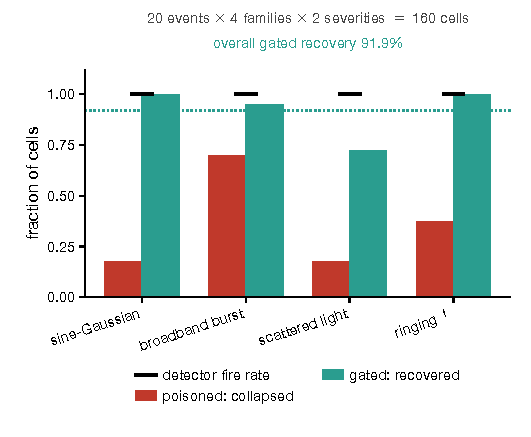
\includegraphics[width=0.6\linewidth]{figures/fig5_synthetic_panel.pdf}
\caption{Synthetic BNS panel: poisoned collapse and gated recovery by family, with the detector fire rate marked.
The dotted line is the overall gated recovery.}
\label{fig:synth}
\end{figure}

\subsection{Ablations}
\label{sec:results-ablation}

Table~\ref{tab:ablation} and Figure~\ref{fig:ablation} isolate the contribution of each design choice on $N=16$ hardening cells (drawn at the two higher severities, 6 and 10, so the absolute rates are lower than on the full grid).
The full recipe (\texttt{adapt\_full}: gate + matched-delta + original ASD) recovers $81.3\%$ with a median $\dL$ of $34.6\,\mathrm{Mpc}$ against a clean reference of $33.9\,\mathrm{Mpc}$.
Full FFT replacement with the original ASD (\texttt{fft\_replace}) recovers $0\%$ and collapses to the prior floor in every cell.
This arm uses the same detector, the same gates, and the same ASD as the full recipe; the only difference is whether the packaged strain is overwritten by $\mathcal{F}[x_{\mathrm{g}}]$ or corrected by $\mathcal{F}[x_{\mathrm{g}}]-\mathcal{F}[x]$.
Time-domain gating alone is therefore not the fix; it is a necessary step that becomes useless if the frequency-domain rewrite discards the packaging residual $\varepsilon$ of Section~\ref{sec:matched-delta}.
Gating with a Welch ASD recomputed on the gated segment (\texttt{gate\_welch}) recovers only $12.5\%$.
Contaminated strain with the original ASD but no gate (\texttt{glitch\_orig\_asd}) likewise recovers $12.5\%$.
Poisoning with a Welch ASD and no gate recovers $6.3\%$.
These contrasts identify matched-delta reconstruction \emph{and} original-ASD retention as jointly necessary.

\begin{table}[t]
\centering
\caption{Ablation on the method-hardening panel ($N=16$ cells per arm).
``Recovers'' is the clean-like recovery rate; ``Collapse'' is the poisoned-style $\dL$ collapse rate after the arm is applied.}
\label{tab:ablation}
\begin{tabular}{lccc}
\toprule
Arm & Recovers & Collapse & Median $\dL$ [Mpc] \\
\midrule
\texttt{adapt\_full}       & 0.813 & 0.125 & 34.6 \\
\texttt{fft\_replace}      & 0.000 & 1.000 & 10.0 \\
\texttt{gate\_welch}       & 0.125 & 0.625 & 10.1 \\
\texttt{glitch\_orig\_asd} & 0.125 & 0.813 & 27.8 \\
\texttt{poison\_welch}     & 0.063 & 0.625 & 10.5 \\
\bottomrule
\end{tabular}
\end{table}

\begin{figure}[t]
\centering
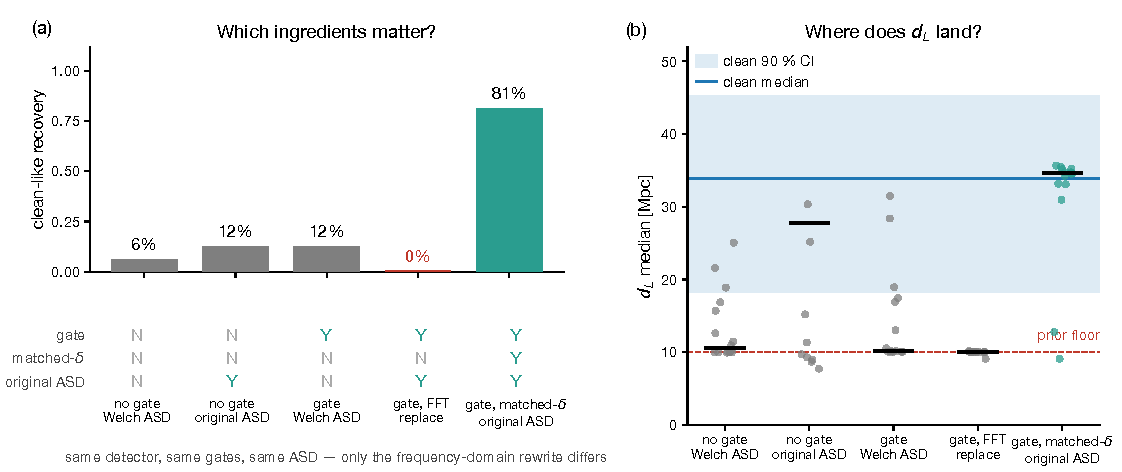
\includegraphics[width=\linewidth]{figures/fig6_ablation.pdf}
\caption{Ablation of reconstruction and ASD policy on the hardening panel.
Left: clean-like recovery rate per arm.
Right: median $\dL$ across cells against the clean median and 90\% interval; three of the five arms sit on the $10\,\mathrm{Mpc}$ prior floor.
Matched-delta reconstruction with the original ASD is the only arm that recovers.}
\label{fig:ablation}
\end{figure}

\begin{figure}[t]
\centering
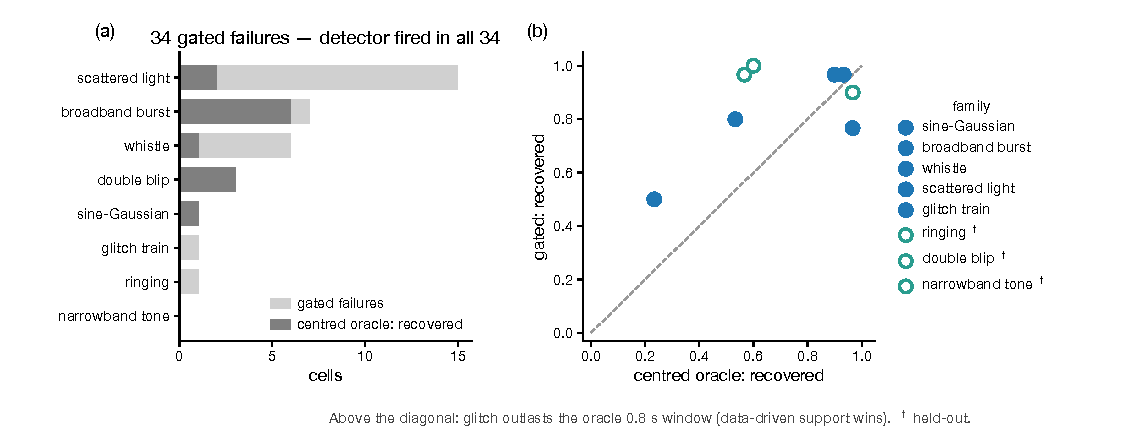
\includegraphics[width=\linewidth]{figures/fig7_oracle_gap.pdf}
\caption{Localization versus extent on the GW170817 grid.
Left: the 34 gated failures by family, and how many the centred fixed-width oracle rescues; the detector fired in all 34.
Right: per-family recovery of the detector-driven gate against the oracle; families above the diagonal are those whose glitches outlast the oracle's $0.8\,\mathrm{s}$ window (green: held-out).}
\label{fig:oracle}
\end{figure}

\subsection{Cost of a false gate}
\label{sec:results-cleangate}

The detector's zero fire rate on 50 clean draws is one safeguard; the other is what a gate costs when it does fire on clean data.
Forcing 25 $\pm0.4\,\mathrm{s}$ gates into glitch-free GW170817 data (20 on H1, 5 on H1 and L1 simultaneously) and passing them through the full front-end removes on average $0.65\%$ of in-band power, produces no collapse, and satisfies the recovery criterion in $23/25$ cases.
The cost is not zero: the mean absolute $\dL$-median shift is $3.8\,\mathrm{Mpc}$ and the largest $\dL$ JS divergence against the clean posterior is $0.24\,\mathrm{nat}$ (the clean-versus-clean resampling null is $0.04\,\mathrm{nat}$ at $n=512$), with the largest shifts for gates closest to coalescence.
A false trigger therefore costs a modest, bounded broadening and shift of the distance posterior, an order of magnitude smaller than the collapse it guards against, which is why the operating threshold is set for a low clean fire rate rather than maximal sensitivity.

\subsection{Runtime}
\label{sec:results-runtime}

On the hardening panel, mean inject-and-detect time is $3.16\,\mathrm{s}$, gated rebuild of all arms is $0.03\,\mathrm{s}$, and adapt PE sampling is $1.52\,\mathrm{s}$ (CPU; $n=512$ samples), compared with $1.46\,\mathrm{s}$ for poisoned PE alone.
Most of the inject-and-detect time is spectrogram construction in a research driver; the detector forward pass and the rebuild together take well under $0.1\,\mathrm{s}$.
The front-end therefore adds a small constant overhead to a single frozen-network evaluation and remains compatible with low-latency budgets once the detector runs on streaming crops~\cite{Chaudhary2024latency,Morisaki2023rapid}.
All timings are single-laptop CPU measurements.

%% =====================================================================
\section{Discussion}
\label{sec:discussion}
%% =====================================================================

\subsection{Why the recipe works}
\label{sec:why}

\DINGOBNS is trained to interpret frequency-domain strain that has been conditioned and whitened in one specific way, and it has no mechanism for reporting that an input lies outside that distribution.
The collapse we observe is the behaviour of a flow pushed off-support: the distance marginal, which for a BNS is set largely by the overall signal amplitude relative to the whitening ASD, is driven to whichever prior boundary best explains the excess of whitened power, and the interval shrinks because the flow is confident within its own coordinates.
That the threshold is set by $\rho_w$ and not by the glitch's position within the segment (Section~\ref{sec:results-threshold}) is consistent with this account, as is the morphology dependence among real glitches: Koi-Fish glitches concentrate broadband power in the $30$--$300\,\mathrm{Hz}$ band that carries most of the BNS SNR, whereas whistles and scattered light place comparable $\rho_w$ where the network is less sensitive.
Two ingredients are needed to bring the input back.
Gating removes the worst time support, but the way the gated data are written back into the package determines whether the network recognizes the result.
A naive FFT rewrite replaces the packaged strain with an approximation that differs from it by a residual $\varepsilon$ encoding windowing, phase, and calibration conventions; that residual is invisible in a strain plot but is, empirically, enough to collapse every cell.
The matched-delta update of Eq.~\eqref{eq:matched-delta} propagates only the excised glitch and leaves $\varepsilon$ untouched.
Restoring the original ASD is the frequency-domain counterpart: a Welch ASD recomputed on gated data encodes the gate as a spectral feature and moves the whitening map outside the training support~\cite{Wildberger2023psd,Chatziioannou2019psd}.
Table~\ref{tab:ablation} is the empirical form of this account: every arm that breaks either packaging or whitening fails; the arm that preserves both succeeds.
The practical lesson generalizes beyond \DINGOBNS: any amortized estimator should be fed corrections to its packaged input rather than re-derivations of it.

\subsection{Failure modes}
\label{sec:failures}

Section~\ref{sec:results-oracle} establishes that the residual failures are a problem of gate extent.
Scattered-light-like arches are the principal case: they are extended in time and concentrated at low frequency, so even the detector's adaptive support leaves residual power that still collapses $\dL$, and the centred oracle does worse still ($23\%$).
Because the detector fired in every failing cell, the detection stage is not the bottleneck, and the obvious next iteration is a gate whose extent is set by the measured excess rather than by a fixed dilation: multi-scale or frequency-dependent gates, or a hybrid in which long low-frequency glitches are handed to wavelet subtraction~\cite{Cornish2015bayeswave,Hourihane2022overlap} while short ones are gated.
The oracle comparison also shows the cost of over-excision: on compact bursts the perfectly centred window beats the detector's dilated support, so widening the dilation to help scattered light would trade against signal preservation on blips.
A per-family or per-duration gate policy is the natural resolution.

\subsection{Relation to likelihood-based mitigation and retraining}
\label{sec:compare}

BayesWave-style joint modelling remains the gold standard when a likelihood is available and latency is secondary~\cite{Davis2022subtract,Ghonge2024efficacy}.
Retraining or glitch-augmenting the density estimator~\cite{Sun2024ttsf,Xiong2025robust} improves intrinsic robustness but requires control of the training stack and careful monitoring of clean-data calibration.
The front-end here is complementary: it protects a frozen production checkpoint at modest overhead and can sit in front of either neural or conventional samplers.
Where glitches are long, coherent across detectors, or morphologically unknown, likelihood-based subtraction or joint signal--glitch inference~\cite{Malz2025joint} remains preferable.

\subsection{Limitations}
\label{sec:limits}

The real-glitch panel transplants O3 excerpts into the GW170817 segment through whitening, STFT thresholding, and re-colouring, which removes the glitch's own noise context and may attenuate low-amplitude structure; the noise-only control bounds one side of this effect but not the other.
The loudest real bin contains only Koi-Fish glitches (five triggers, fifteen cells), and the ``Extremely Loud'' class that dominates the catalogue tail was not sampled, so the collapse rate on real glitches above SNR 300 is a Koi-Fish rate, not a population rate.
Only one real event packaging (GW170817) is used, supplemented by the synthetic panel; gate dilation is fixed; and no importance-sampling correction of the gated posterior is applied~\cite{Dax2023is}, although the importance-sampling efficiency of the gated control package is comparable to the clean one.
The clean-gate control shows that a false trigger is not free, so the detector threshold, not the front-end, sets the operating point.
The detector is trained on the same synthetic generator used for held-in evaluation, although held-out families partially probe generalization.
Runtimes are CPU/MPS measurements for research drivers, not a profiled low-latency deployment.
Extension to binary black hole DINGO networks and to simultaneous multi-detector glitches is left to future work.

\subsection{Deployment considerations}
\label{sec:deploy}

For low-latency use the detector should run continuously on overlapping STFT crops with a calibrated false-positive rate (here $1\%$ at training calibration; $0\%$ on the 50-draw event audit), and, given the threshold measured here, gating could be reserved for triggers whose estimated $\rho_w$ exceeds a few hundred, below which the network is robust and a gate can only cost signal.
Gates should be broadcast to the event packager only when a trigger coincides with a candidate coalescence window, minimizing unnecessary signal excision.
Logging detector probabilities, gate windows, and ASD provenance alongside posterior samples would preserve data-quality audit trails analogous to those used in O3 glitch subtraction campaigns~\cite{Davis2022subtract}.

%% =====================================================================
\section{Conclusion}
\label{sec:conclusion}
%% =====================================================================

The frozen \DINGOBNS checkpoint is more robust to transient glitches than a naive stress test would suggest, and less robust than a low-latency pipeline can afford.
Real O3 glitches at native loudness leave the posterior untouched below Omicron SNR 100; above a whitened optimal SNR of a few thousand, roughly the loudest tenth of confidently classified O3 triggers, the distance posterior collapses to a prior boundary with a credible interval far too narrow to signal the failure, independently of where the glitch sits in the segment.
A lightweight detect--gate--rebuild front-end (STFT detection, Tukey gating, matched-delta frequency-domain reconstruction, and retention of the original analysis ASDs) restores clean-like posteriors in $99\%$ of real-glitch cells, $86\%$ of a 240-cell loud-glitch stress grid, and $92\%$ of a synthetic BNS panel, without modifying network weights and on morphologies the detector was never trained on.
Ablations show that matched-delta reconstruction with the original ASD is indispensable; full FFT replacement recovers nothing, and the gap between the two isolates a packaging residual the frozen network cannot tolerate.
A fixed-width oracle with perfect knowledge of the glitch time recovers fewer cells than the detector-driven gate, so the remaining failures are a matter of gate extent, and a clean-gate control bounds the price of a false trigger.
The accompanying software and archived results make every number reproducible and the front-end available for integration into low-latency neural inference stacks.

\section*{CRediT authorship contribution statement}
\textbf{Jayant Kumar:} Conceptualization, Methodology, Software, Validation, Formal analysis, Investigation, Data curation, Writing (original draft), Writing (review \& editing), Visualization.

\section*{Declaration of competing interest}
The author declares that he has no known competing financial interests or personal relationships that could have appeared to influence the work reported in this paper.

\section*{Data availability}
Open strain data are available from the Gravitational Wave Open Science Center~\cite{Abbott2021opendata,Abbott2023opendata}.
The \DINGOBNS demonstration model is obtained from the upstream DINGO release~\cite{Dax2025bns}.
Source code, the STFT detector checkpoint, and archived result summaries for this study are available at \url{https://github.com/Jayant-Kumar17/glitch-robust-dingo-bns} (release v1.1.0; Zenodo DOI to be added on acceptance).
Every number in the tables is read from the archived JSON and CSV summaries under \texttt{results/}, and Figures~\ref{fig:pipeline}--\ref{fig:oracle} are regenerated from them by \texttt{paper/make\_figures.py}, \texttt{paper/make\_figures\_t5.py}, and \texttt{examples/paper\_figures\_2\_3.py}.
The Gravity Spy O3 classifications are from Zenodo record 5649212~\cite{Glanzer2023gravityspy}.

\section*{Acknowledgements}
This research has made use of data or software obtained from the Gravitational Wave Open Science Center (\url{https://gwosc.org}), a service of the LIGO Scientific Collaboration, the Virgo Collaboration, and KAGRA.
This material is based upon work supported by NSF's LIGO Laboratory, which is a major facility fully funded by the National Science Foundation.



\appendix

\section{Glitch family parameter ranges}
\label{app:glitch}

Held-in families, used for detector training and primary evaluation, are \texttt{sine\_gaussian}, \texttt{broadband\_burst}, \texttt{whistle}, \texttt{scattered\_light}, and \texttt{glitch\_train}.
Held-out families reserved for generalization tests are \texttt{ringing}, \texttt{double\_blip}, and \texttt{narrowband\_tone}.
Each draw samples a relative peak time within the analysis crop, an in-band severity, and family-specific shape parameters (central frequency, quality factor, chirp rate, envelope duration, or inter-blip delay) from broad uniform or log-uniform ranges implemented in \texttt{adapt.glitch\_augmentation}.
Injections are added to a single interferometer's time-domain strain and propagated to the frequency-domain package with the configured ASD policy.
Exact sampling ranges are versioned in the accompanying repository configuration files.

\section{STFT detector architecture and training}
\label{app:detector}

The detector is a convolutional encoder over whitened spectrograms of shape $(B,C,T,F)$ with $T=32$, $F=128$, and $C$ equal to the number of interferometer channels in the stack.
A stem convolution (32 base channels) is followed by two residual-style blocks that pool only along frequency, preserving time alignment; a $1\times 1$ convolution then emits per-interferometer time-bin logits.
The final bias is initialized to $-4$ so that a randomly initialized network is silent on clean data.
Training uses binary cross-entropy with positive-bin weight $3.0$, Adam at learning rate $10^{-3}$, batch size 16, 100 steps per epoch, and of order 20--30 epochs.
Thresholds are calibrated on a clean-containing calibration set to a target false-positive rate of $0.01$.
The released checkpoint reports a best validation score of $\approx 0.77$ at threshold $\approx 0.46$; event-level analyses optionally raise the threshold (e.g.\ $\approx 0.73$ on the GW170817 grid) after a per-event clean audit.

\section{Reproduction commands}
\label{app:repro}

With the official \DINGOBNS demonstration assets and the released detector checkpoint installed,
\begin{verbatim}
conda activate adapt_env
pip install -e .
export PYTHONPATH=src:examples
export KMP_DUPLICATE_LIB_OK=TRUE

python -u examples/official_control.py \
  --outdir results/dingo_official_control
python -u examples/honest_excision.py \
  --outdir results/excision_honest
python -u examples/stress_gw170817.py \
  --seed 0 --n-seeds-per-cell 5 \
  --num-samples 512 --outdir results/stress_test_excision_v1
python -u examples/stress_synthetic_bns.py \
  --outdir results/stress_test_synthetic_bns_v1
python -u examples/method_hardening.py \
  --num-samples 512 --outdir results/journal_method_hardening_v1
python -u examples/clean_gate_control.py \
  --outdir results/clean_gate_control_v1
python -u examples/collapse_threshold.py --seed 0 \
  --num-samples 512 --n-seeds 5 \
  --outdir results/collapse_threshold_v1
python -u examples/collapse_threshold.py --extend-low-rho \
  --outdir results/collapse_threshold_v1
python -u examples/stress_real_glitches.py --seed 0 \
  --num-samples 512 --outdir results/stress_real_glitches_v2
python -u examples/loudness_audit.py \
  --outdir results/loudness_audit_v1
\end{verbatim}
Archived summaries under \texttt{results/*/} are the numerical source for Tables~\ref{tab:real}--\ref{tab:ablation}.

%% =====================================================================
%% Bibliography
%% =====================================================================
\ifusebibtex
  \bibliographystyle{elsarticle-num}
  \bibliography{refs}
\else
\begin{thebibliography}{99}

\bibitem{Abbott2016noise}
B.~P. Abbott et al. (LIGO Scientific Collaboration and Virgo Collaboration),
Characterization of transient noise in Advanced LIGO relevant to gravitational wave signal GW150914,
Classical and Quantum Gravity 33~(13) (2016) 134001,
doi:10.1088/0264-9381/33/13/134001.

\bibitem{Abbott2017gw170817}
B.~P. Abbott et al. (LIGO Scientific Collaboration and Virgo Collaboration),
GW170817: Observation of Gravitational Waves from a Binary Neutron Star Inspiral,
Physical Review Letters 119~(16) (2017) 161101,
doi:10.1103/PhysRevLett.119.161101.

\bibitem{Abbott2017mma}
B.~P. Abbott et al. (LIGO Scientific Collaboration, Virgo Collaboration and others),
Multi-messenger Observations of a Binary Neutron Star Merger,
The Astrophysical Journal Letters 848~(2) (2017) L12,
doi:10.3847/2041-8213/aa91c9.

\bibitem{Abbott2019gwtc1}
B.~P. Abbott et al. (LIGO Scientific Collaboration and Virgo Collaboration),
GWTC-1: A Gravitational-Wave Transient Catalog of Compact Binary Mergers Observed by LIGO and Virgo during the First and Second Observing Runs,
Physical Review X 9~(3) (2019) 031040,
doi:10.1103/PhysRevX.9.031040.

\bibitem{Abbott2020guide}
B.~P. Abbott et al. (LIGO Scientific Collaboration and Virgo Collaboration),
A guide to LIGO--Virgo detector noise and extraction of transient gravitational-wave signals,
Classical and Quantum Gravity 37~(5) (2020) 055002,
doi:10.1088/1361-6382/ab685e.

\bibitem{Abbott2021opendata}
R.~Abbott et al. (LIGO Scientific Collaboration and Virgo Collaboration),
Open data from the first and second observing runs of Advanced LIGO and Advanced Virgo,
SoftwareX 13 (2021) 100658,
doi:10.1016/j.softx.2021.100658.

\bibitem{Abbott2023opendata}
R.~Abbott et al. (LIGO Scientific Collaboration, Virgo Collaboration and KAGRA Collaboration),
Open Data from the Third Observing Run of LIGO, Virgo, KAGRA, and GEO,
The Astrophysical Journal Supplement Series 267~(2) (2023) 29,
doi:10.3847/1538-4365/acdc9f.

\bibitem{Ashton2019bilby}
G.~Ashton et al.,
BILBY: A User-friendly Bayesian Inference Library for Gravitational-wave Astronomy,
The Astrophysical Journal Supplement Series 241~(2) (2019) 27,
doi:10.3847/1538-4365/ab06fc.

\bibitem{Ashton2023gp}
G.~Ashton,
Gaussian processes for glitch-robust gravitational-wave astronomy,
Monthly Notices of the Royal Astronomical Society 520~(2) (2023) 2983--2994,
doi:10.1093/mnras/stad341.

\bibitem{Bahaadini2018}
S.~Bahaadini, V.~Noroozi, N.~Rohani, S.~Coughlin, M.~Zevin, J.~R. Smith, V.~Kalogera, A.~Katsaggelos,
Machine learning for Gravity Spy: Glitch classification and dataset,
Information Sciences 444 (2018) 172--186,
doi:10.1016/j.ins.2018.02.068.

\bibitem{Cabero2019blip}
M.~Cabero et al.,
Blip glitches in Advanced LIGO data,
Classical and Quantum Gravity 36~(15) (2019) 155010,
doi:10.1088/1361-6382/ab2e14.

\bibitem{Chatziioannou2019psd}
K.~Chatziioannou, C.-J. Haster, T.~B. Littenberg, W.~M. Farr, S.~Ghonge, M.~Millhouse, J.~A. Clark, N.~Cornish,
Noise spectral estimation methods and their impact on gravitational wave measurement of compact binary mergers,
Physical Review D 100~(10) (2019) 104004,
doi:10.1103/PhysRevD.100.104004.

\bibitem{Chaudhary2024latency}
S.~S. Chaudhary et al.,
Low-latency gravitational wave alert products and their performance at the time of the fourth LIGO--Virgo--KAGRA observing run,
Proceedings of the National Academy of Sciences 121~(18) (2024) e2316474121,
doi:10.1073/pnas.2316474121.

\bibitem{Cornish2015bayeswave}
N.~J. Cornish, T.~B. Littenberg,
BayesWave: Bayesian inference for gravitational wave bursts and instrument glitches,
Classical and Quantum Gravity 32~(13) (2015) 135012,
doi:10.1088/0264-9381/32/13/135012.

\bibitem{Cranmer2020sbi}
K.~Cranmer, J.~Brehmer, G.~Louppe,
The frontier of simulation-based inference,
Proceedings of the National Academy of Sciences 117~(48) (2020) 30055--30062,
doi:10.1073/pnas.1912789117.

\bibitem{Davis2021detchar}
D.~Davis et al.,
LIGO detector characterization in the second and third observing runs,
Classical and Quantum Gravity 38~(13) (2021) 135014,
doi:10.1088/1361-6382/abfd85.

\bibitem{Davis2022subtract}
D.~Davis, T.~B. Littenberg, I.~M. Romero-Shaw, M.~Millhouse, J.~McIver, F.~Di Renzo, G.~Ashton,
Subtracting glitches from gravitational-wave detector data during the third LIGO--Virgo observing run,
Classical and Quantum Gravity 39~(24) (2022) 245013,
doi:10.1088/1361-6382/aca238.

\bibitem{Dax2021dingo}
M.~Dax, S.~R. Green, J.~Gair, J.~H. Macke, A.~Buonanno, B.~Sch\"olkopf,
Real-Time Gravitational Wave Science with Neural Posterior Estimation,
Physical Review Letters 127~(24) (2021) 241103,
doi:10.1103/PhysRevLett.127.241103.

\bibitem{Dax2022gnpe}
M.~Dax, S.~R. Green, J.~Gair, M.~Deistler, B.~Sch\"olkopf, J.~H. Macke,
Group equivariant neural posterior estimation,
in: International Conference on Learning Representations, 2022.

\bibitem{Dax2023is}
M.~Dax, S.~R. Green, J.~Gair, M.~P\"urrer, J.~Wildberger, J.~H. Macke, A.~Buonanno, B.~Sch\"olkopf,
Neural Importance Sampling for Rapid and Reliable Gravitational-Wave Inference,
Physical Review Letters 130~(17) (2023) 171403,
doi:10.1103/PhysRevLett.130.171403.

\bibitem{Dax2025bns}
M.~Dax, S.~R. Green, J.~Gair, N.~Gupte, M.~P\"urrer, V.~Raymond, J.~Wildberger, J.~H. Macke, A.~Buonanno, B.~Sch\"olkopf,
Real-time inference for binary neutron star mergers using machine learning,
Nature 639~(8053) (2025) 49--53,
doi:10.1038/s41586-025-08593-z.

\bibitem{Durkan2019nsf}
C.~Durkan, A.~Bekasov, I.~Murray, G.~Papamakarios,
Neural Spline Flows,
in: Advances in Neural Information Processing Systems, Vol.~32, 2019.

\bibitem{Edy2021mismodel}
O.~Edy, A.~Lundgren, L.~K. Nuttall,
Issues of mismodeling gravitational-wave data for parameter estimation,
Physical Review D 103~(12) (2021) 124061,
doi:10.1103/PhysRevD.103.124061.

\bibitem{George2018dnn}
D.~George, E.~A. Huerta,
Deep Neural Networks to Enable Real-time Multimessenger Astrophysics,
Physical Review D 97~(4) (2018) 044039,
doi:10.1103/PhysRevD.97.044039.

\bibitem{Ghonge2024efficacy}
S.~Ghonge et al.,
Assessing and mitigating the impact of glitches on gravitational-wave parameter estimation: A model agnostic approach,
Physical Review D 110~(12) (2024) 122002,
doi:10.1103/PhysRevD.110.122002.

\bibitem{Glanzer2023gravityspy}
J.~Glanzer et al.,
Data quality up to the third observing run of advanced LIGO: Gravity Spy glitch classifications,
Classical and Quantum Gravity 40~(6) (2023) 065004,
doi:10.1088/1361-6382/acb633.

\bibitem{Green2021npe}
S.~R. Green, J.~Gair,
Complete parameter inference for GW150914 using deep learning,
Machine Learning: Science and Technology 2~(3) (2021) 03LT01,
doi:10.1088/2632-2153/abfaed.

\bibitem{Greenberg2019snpe}
D.~Greenberg, M.~Nonnenmacher, J.~Macke,
Automatic Posterior Transformation for Likelihood-Free Inference,
in: Proceedings of the 36th International Conference on Machine Learning, Vol.~97, PMLR, 2019, pp.~2404--2414.

\bibitem{Harris1978windows}
F.~J. Harris,
On the use of windows for harmonic analysis with the discrete Fourier transform,
Proceedings of the IEEE 66~(1) (1978) 51--83,
doi:10.1109/PROC.1978.10837.

\bibitem{Harris2020numpy}
C.~R. Harris et al.,
Array programming with NumPy,
Nature 585 (2020) 357--362,
doi:10.1038/s41586-020-2649-2.

\bibitem{Hourihane2022overlap}
S.~Hourihane, K.~Chatziioannou, M.~Wijngaarden, D.~Davis, T.~Littenberg, N.~Cornish,
Accurate modeling and mitigation of overlapping signals and glitches in gravitational-wave data,
Physical Review D 106~(4) (2022) 042006,
doi:10.1103/PhysRevD.106.042006.

\bibitem{Lin1991jsd}
J.~Lin,
Divergence measures based on the Shannon entropy,
IEEE Transactions on Information Theory 37~(1) (1991) 145--151,
doi:10.1109/18.61115.

\bibitem{Macas2022localization}
R.~Macas et al.,
Impact of noise transients on low latency gravitational-wave event localization,
Physical Review D 105~(10) (2022) 103021,
doi:10.1103/PhysRevD.105.103021.

\bibitem{Macleod2021gwpy}
D.~M. Macleod, J.~S. Areeda, S.~B. Coughlin, T.~J. Massinger, A.~L. Urban,
GWpy: A Python package for gravitational-wave astrophysics,
SoftwareX 13 (2021) 100657,
doi:10.1016/j.softx.2021.100657.

\bibitem{Malz2025joint}
A.-K. Malz, J.~Veitch,
Joint inference for gravitational wave signals and glitches using a data-informed glitch model,
Physical Review D 112~(2) (2025) 024071,
doi:10.1103/fp4b-mvzx.

\bibitem{Merritt2021glitschen}
J.~Merritt, B.~Farr, R.~Hur, B.~Edelman, Z.~Doctor,
Transient glitch mitigation in Advanced LIGO data with glitschen,
Physical Review D 104~(10) (2021) 102004,
doi:10.1103/PhysRevD.104.102004.

\bibitem{Morisaki2023rapid}
S.~Morisaki, R.~Smith, L.~Tsukada, S.~Sachdev, S.~Stevenson, C.~Talbot, A.~Zimmerman,
Rapid localization and inference on compact binary coalescences with the Advanced LIGO--Virgo--KAGRA gravitational-wave detector network,
Physical Review D 108~(12) (2023) 123040,
doi:10.1103/PhysRevD.108.123040.

\bibitem{Mozzon2020dynamic}
S.~Mozzon, L.~K. Nuttall, A.~Lundgren, T.~Dent, S.~Kumar, A.~H. Nitz,
Dynamic normalization for compact binary coalescence searches in non-stationary noise,
Classical and Quantum Gravity 37~(21) (2020) 215014,
doi:10.1088/1361-6382/abac6c.

\bibitem{Nuttall2018transient}
L.~K. Nuttall,
Characterizing transient noise in the LIGO detectors,
Philosophical Transactions of the Royal Society A 376~(2120) (2018) 20170286,
doi:10.1098/rsta.2017.0286.

\bibitem{Papamakarios2016mdn}
G.~Papamakarios, I.~Murray,
Fast $\varepsilon$-free Inference of Simulation Models with Bayesian Conditional Density Estimation,
in: Advances in Neural Information Processing Systems, Vol.~29, 2016.

\bibitem{Papamakarios2021review}
G.~Papamakarios, E.~Nalisnick, D.~J. Rezende, S.~Mohamed, B.~Lakshminarayanan,
Normalizing Flows for Probabilistic Modeling and Inference,
Journal of Machine Learning Research 22~(57) (2021) 1--64.

\bibitem{Pankow2018mitigation}
C.~Pankow et al.,
Mitigation of the instrumental noise transient in gravitational-wave data surrounding GW170817,
Physical Review D 98~(8) (2018) 084016,
doi:10.1103/PhysRevD.98.084016.

\bibitem{Paszke2019pytorch}
A.~Paszke et al.,
PyTorch: An Imperative Style, High-Performance Deep Learning Library,
in: Advances in Neural Information Processing Systems, Vol.~32, 2019.

\bibitem{Payne2022gw200129}
E.~Payne, S.~Hourihane, J.~Golomb, R.~Udall, D.~Davis, K.~Chatziioannou,
Curious case of GW200129: Interplay between spin-precession inference and data-quality issues,
Physical Review D 106~(10) (2022) 104017,
doi:10.1103/PhysRevD.106.104017.

\bibitem{Powell2018glitchpe}
J.~Powell,
Parameter estimation and model selection of gravitational wave signals contaminated by transient detector noise glitches,
Classical and Quantum Gravity 35~(15) (2018) 155017,
doi:10.1088/1361-6382/aacf18.

\bibitem{Razzano2018cnn}
M.~Razzano, E.~Cuoco,
Image-based deep learning for classification of noise transients in gravitational wave detectors,
Classical and Quantum Gravity 35~(9) (2018) 095016,
doi:10.1088/1361-6382/aab793.

\bibitem{Singer2016bayestar}
L.~P. Singer, L.~R. Price,
Rapid Bayesian position reconstruction for gravitational-wave transients,
Physical Review D 93~(2) (2016) 024013,
doi:10.1103/PhysRevD.93.024013.

\bibitem{Soni2021scattered}
S.~Soni et al.,
Reducing scattered light in LIGO's third observing run,
Classical and Quantum Gravity 38~(2) (2021) 025016,
doi:10.1088/1361-6382/abc906.

\bibitem{Sun2024ttsf}
T.-Y. Sun, C.-Y. Xiong, S.-J. Jin, Y.-X. Wang, J.-F. Zhang, X.~Zhang,
Efficient parameter inference for gravitational wave signals in the presence of transient noises using temporal and time-spectral fusion normalizing flow,
Chinese Physics C 48~(4) (2024) 045108,
doi:10.1088/1674-1137/ad2a5f.

\bibitem{Talbot2020psd}
C.~Talbot, E.~Thrane,
Gravitational-wave astronomy with an uncertain noise power spectral density,
Physical Review Research 2~(4) (2020) 043298,
doi:10.1103/PhysRevResearch.2.043298.

\bibitem{Usman2016pycbc}
S.~A. Usman et al.,
The PyCBC search for gravitational waves from compact binary coalescence,
Classical and Quantum Gravity 33~(21) (2016) 215004,
doi:10.1088/0264-9381/33/21/215004.

\bibitem{Virtanen2020scipy}
P.~Virtanen et al.,
SciPy 1.0: fundamental algorithms for scientific computing in Python,
Nature Methods 17 (2020) 261--272,
doi:10.1038/s41592-019-0686-2.

\bibitem{Welch1967}
P.~D. Welch,
The use of fast Fourier transform for the estimation of power spectra: A method based on time averaging over short, modified periodograms,
IEEE Transactions on Audio and Electroacoustics 15~(2) (1967) 70--73,
doi:10.1109/TAU.1967.1161901.

\bibitem{Wildberger2023psd}
J.~Wildberger, M.~Dax, S.~R. Green, J.~Gair, M.~P\"urrer, J.~H. Macke, A.~Buonanno, B.~Sch\"olkopf,
Adapting to noise distribution shifts in flow-based gravitational-wave inference,
Physical Review D 107~(8) (2023) 084046,
doi:10.1103/PhysRevD.107.084046.

\bibitem{Xiong2025robust}
C.-Y. Xiong, T.-Y. Sun, J.-F. Zhang, X.~Zhang,
Robust inference of gravitational wave source parameters in the presence of noise transients using normalizing flows,
Physical Review D 111~(2) (2025) 024019,
doi:10.1103/PhysRevD.111.024019.

\bibitem{Zackay2021nongaussian}
B.~Zackay, T.~Venumadhav, J.~Roulet, L.~Dai, M.~Zaldarriaga,
Detecting gravitational waves in data with non-stationary and non-Gaussian noise,
Physical Review D 104~(6) (2021) 063034,
doi:10.1103/PhysRevD.104.063034.

\bibitem{Zevin2017gravityspy}
M.~Zevin et al.,
Gravity Spy: integrating advanced LIGO detector characterization, machine learning, and citizen science,
Classical and Quantum Gravity 34~(6) (2017) 064003,
doi:10.1088/1361-6382/aa5cea.

\end{thebibliography}
\fi

\end{document}
